\chapter{Usability Testing}
When we started this project the main reason was to simplify the administration systems to one single interface. So that there is only one code base and only one interface for the user to learn.\\
The first part should be given by default because we use a specialized system to run PHP code on the tablet. The system is called PAW \citep{paw} and is still in its beta phase.\\
The second part is the tricky part. There is only one interface to use, but it must be easy to learn and use so that the system does not have to be reworked.\\
That is why we have performed a usability test.\\
\\

%How did we do the test
	%Who was where
	%The simularity of the questions
The test was performed in Cassiopeias usability lab, where we had logged the computer onto our website. The setup of the usability lab is as displayed on figure \ref{fig:usabilitylab}. We did not use the second room.\\
Each test person was lead into the test room, offered a cup of coffee and then we started the prepared briefing, everyone was given the same briefing and we asked them to sign a consent form that they were being tapped for research purposes.\\
After this we asked them to execute a set of assignments within the system, always the same assignments, designed to lead them around the whole active system. \fix{Add a refference to appendix with questions and briefing}\\
We had the same one person sit in the room to assist the user, both to give them their assignment and to tell them when they had completed it. All assignments was kept very short, as to not disturb the user more then needed.\\
When the user had completed all the assignments we had the two men that sat in the control room come and help ask questions to the test person about some of the ways the test person used the system.\\
\\

\begin{figure}[htbp]
	\centering
		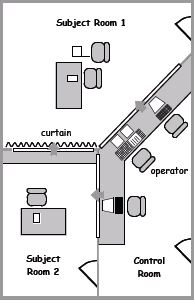
\includegraphics[width=0.40\textwidth]{images/usabilitylab.png}
	\caption{Usability Lab}
	\label{fig:usabilitylab}
\end{figure}

	%Picking the candidates
This test was only performed on 4 persons, this might not sound as many. But being that there is only a few persons in Denmark that will use the administration features that we have designed. We had to make an expert test, and use the gathered data as such. We only had one person available that we thought would use the main system that we have designed, but this person who is responsibly for a kinder garden, is not even high enough up in their system to be using most of the admin features. But this is all we had to go on, as we had no way of contacting the persons who is in a high enough position to be the intended user.\\
So the test was carried out with the one person to be the actual test person, and the 3 others be confirmation test, so that we did not draw conclusions from one test, that could be a result of lacking computer skills or other variables of the same sort.
	
	%The old version
	
%Result of the test
	%Bugs/Errors
		%Severity
\begin{table}[htbp]
	\centering
		\begin{tabular}{|l|l|l|}
			\hline
			Description & Severity & Done\\\hline\hline
			It is not possible to create new categories of Pictos & Critical &\\\hline
			Profile - Restrict QR editing to department manager & Critical &  \\\hline 
			DB Problem - Not possible for all pedagogs to fix pictos for all department children & Critical & \\\hline
			Navigation - The site ''Profiles'' should link to each profile & Critical &\\\hline
			Missing - Unable to remove relations & Critical & \\\hline
			Profile Pic - Accept button is hard to find & Serious &\\\hline
			Profile Pic - Word ''change'' is misleading & Serious &\\\hline
			Navigation - ''Add'' and ''Make'' under Pics Manager is confusing & Serious & \\\hline
			Navigation - Language Support on navigation did not change to danish & Serious & Done\\\hline
			Missing - No Danish language support on the site ''Profiles''& Serious &\\\hline
			Profile - Department should be a link, not editable & Serious & (Done)\\\hline
			Profile - Links from Own Profile relations is missing & Serious & \\\hline
			Profile Pic - GIRAF Logo as Placeholder is misleading  & Cosmetic & Done\\\hline
			Profile Pic - Word ''Edit'' is not informative & Cosmetic &\\\hline
			DB Problem - Own Profile takes too long to load & Cosmetic &  \\\hline
			Navigation - ''Add Relation''  is before ''Create Profile'' & Cosmetic & Done \\\hline
			Standardize button names & Cosmetic & \\\hline
			Logout - Can navigate in system without session & Cosmetic & \\\hline
	\end{tabular}
	\caption{Bugs/Errors Found Under Usability Testing}
	\label{tab:Bugs/Errors}
\end{table}

	%Features
\begin{table}[htbp]
	\centering
		\begin{tabular}{|l|l|}
			\hline
			Description & Done\\\hline\hline
			Make the modal window customizable &\\\hline
			Profile - Press enter to save change &\\\hline
			Pics Manager Make - Add recording feature&\\\hline
			Input forms - Automatic first letter uppercase for name and address&\\\hline  
			Navigation - Add link to ''add relations'' and ''create profile'' in Profiles & \\\hline  
			Pics Manager Make - Directly create picto for child from profile page & \\\hline
			Pics Manager Make - Auto add ''inline-text'' to picto preview. & \\\hline
		\end{tabular}
	\caption{Features Found Under Usability Testing}
	\label{tab:NewFeature}
\end{table}	
	
%What have we already fixed

%What MUST be fixed

%What could be added later - Maybe a refference to Future Work instead?